\documentclass[xcolor=pdftex,table,10pt,yellow,mathserif]{beamer}
\usepackage[3D]{movie15}
\usepackage{array}
\usepackage{amsmath}
\usepackage{algorithm,algorithmic}
\usepackage{tikz}
\usepackage{pgflibraryshapes}  
\usetheme{PSI}
\usetikzlibrary{shapes,arrows,snakes,backgrounds}
%\usetikzlibrary{arrows}
\usepackage[overlay,absolute]{textpos}
\usepackage[latin1]{inputenc}
\usepackage[english]{babel}
\usepackage{listings}

\usepackage{pgfpages}\newcommand{\opal}{\textsc{OPAL}}
\newcommand{\opalt}{\textsc{OPAL-t }}
\newcommand{\opalcycl}{\textsc{OPAL-cycl}}
\newcommand{\opalmap}{\textsc{OPAL-map }}
\newcommand{\opalenv}{\textsc{OPAL-envelop}}

\newcommand{\mad}{\textsc{mad }}
\newcommand{\madnine}{\textsc{mad9 }}
\newcommand{\madninep}{\textsc{mad9p }}
\newcommand{\madeight}{\textsc{mad8 }}

\newcommand{\classic}{\textsc{classic }}
\newcommand{\hfifepart}{\textsc{H5Part }}
\newcommand{\hfifefe}{\textsc{H5FED }}

\renewcommand{\epsilon}{\varepsilon} 
\renewcommand{\vec}[1]{{\bf #1}} 
\newcommand{\dt}[1]{\frac{\partial #1}{\partial t}}
\newcommand{\dtt}[1]{\frac{\partial^2 #1}{\partial t^2}}
\newcommand{\dtvec}[1]{\frac{\partial {\mathbf #1}}{\partial t}}
\newcommand{\dttvec}[1]{\frac{\partial^2 {\mathbf #1}}{\partial t^2}}
\newcommand{\rot}{\vec{\nabla} \wedge }
\renewcommand{\div}{\vec{\nabla} \cdot }

\def\vec#1{\mathbf{#1}}
\def\vecg#1{\boldsymbol{#1}}
\def\norm#1{\| #1 \|} 
\def\tr{^{\!\top}}

\def\curl{{\bf curl}\,}
\def\curlp{{\rm curl}_p\,}
\def\div{{\rm div}\,}
\def\grad{\nabla}
\def\gradp{\nabla_p}
\def\dotp#1#2{\langle#1,#2\rangle}
\def\eps{\varepsilon}

\newcommand{\mat}[1]{\ensuremath{\boldsymbol{#1}}}
\newcommand{\vect}[1]{\ensuremath{\mathbf{#1}}}
\newcommand{\iprod}[2]{\ensuremath{\langle#1,#2\rangle}}
\newcommand{\abs}[1]{\ensuremath{|#1|}}

\newcommand{\Nedelec}{N\'{e}d\'{e}lec}

\newcommand{\id}[1]{\structure{#1}}

\newcommand {\Co}{{\mathbb{C}}}
\newcommand {\Int}{{\mathbb{Z}}}
\newcommand {\Nat}{{\mathbb{N}}}
%
%
\newcommand {\Hcurl}{{H(\mathbf{curl};\Omega)}}
\newcommand {\Hocurl}{{H_0(\mathbf{curl};\Omega)}}
\newcommand {\Hdiv}{{H(\mathrm{div};\Omega)}}
\newcommand {\Hodiv}{{H_0(\mathbf{div};\Omega)}}
%
\renewcommand {\Re}{{\rm I \kern-2pt R}}
\newcommand{\vc}[1]{\mbox{\boldmath $#1$}}
\newcommand {\RM}[1]{\mathrm{#1}}



\TPGrid[4mm,25mm]{10}{5}

\tikzstyle{format} = [draw, thin, fill=blue!20]
\tikzstyle{pblock} = [rectangle, draw, fill=blue!20, text width=6em, text centered, rounded corners, minimum height=0.4em]
\tikzstyle{mblock} = [rectangle, draw, fill=green!20, text width=6em, text centered, rounded corners, minimum height=0.4em]
\tikzstyle{bblock} = [rectangle, draw, fill=gray!20, text width=6em, text centered, rounded corners, minimum height=0.4em]
\tikzstyle{prblock} = [rectangle, draw, fill=red!20, text width=6em, text centered, rounded corners, minimum height=0.4em]
\tikzstyle{rblock} = [rectangle, draw, fill=black!50, text width=6em, text centered, rounded corners, minimum height=0.4em]
\tikzstyle{block} = [rectangle, draw, fill=gray!20, text centered, rounded corners]
\tikzstyle{decision} = [diamond, draw, fill=blue!20, text width=4.5em, text badly centered, node distance=3cm, inner sep=0pt]
\tikzstyle{medium} = [ellipse, draw, thin, fill=green!20, minimum height=2.5em]
\tikzstyle{cloud} = [draw, ellipse,fill=red!20, node distance=3cm, minimum height=2em]
\tikzstyle{line} = [draw, -latex']
\tikzstyle{emptyblock} = [rectangle]
\tikzstyle{progblock} = [rectangle, draw, fill=yellow!20, text width=6em, text centered, minimum height=0.4em]
\tikzstyle{null} = [rectangle, fill=blue!0, text width=6em, text centered, rounded corners, minimum height=0.4em]




% Figure 1
\tikzstyle{f1pblock} = [rectangle, draw, fill=blue!20, text width=5em, text centered, rounded corners, minimum height=0.4em]
\tikzstyle{f1pblockr} = [rectangle, draw, fill=red!20, text width=5em, text centered, rounded corners, minimum height=0.4em]
\tikzstyle{f1pblockw} = [rectangle, draw, text width=5em, text centered, rounded corners, minimum height=0.4em]
\tikzstyle{f1rblock} = [rectangle, draw, fill=gray!50, text width=10em, text centered, rounded corners, minimum height=0.4em]
\tikzstyle{f1medium} = [ellipse, draw, fill=green!20, text width=5em, text centered, rounded corners, minimum height=0.4em]
\tikzstyle{f1mediumr} = [ellipse, draw, thin, fill=red!20, minimum height=2.5em]
\tikzstyle{f1line} = [draw, -latex']
\tikzstyle{f1null} = [rectangle, fill=blue!0, text width=6em, text centered, rounded corners, minimum height=0.4em]



\mode<presentation>
{
  \usepackage{pgf}
  \usepackage{hyperref}
  \setbeamercovered{transparent}
  \setbeamercovered{transparent}  
}


\AtBeginSection[]
{
  \begin{frame}<beamer>
    \frametitle{Outline}
    \tableofcontents[currentsection,hideothersubsections]
  \end{frame}
}

\AtBeginSubsection[]
{
  \begin{frame}<beamer>
    \frametitle{Outline}
    \tableofcontents[currentsection,currentsubsection]
  \end{frame}
}

\title{OPAL - Object Oriented Parallel Accelerator Simulation Framework for Present and Future Modeling Challenges}

\author{A. Adelmann (PSI-AMAS) \\ Acknowledgments: Y. Ineichen Ch. Kraus (PSI) Y. Bi, J. Yang (CIAE) \& S. Russel (LANL)}

\date{MS118 SIAM AM 16.\ July 2010}



\titlegraphic{
%      
\includegraphics[width=10cm]{./amas1} \\
 }


\begin{document}
\frame{
\maketitle
}

\begin{frame}
	  \frametitle{Outline}
	  \tableofcontents
	\end{frame}

\section{Motivation \& Problem Setup}
\begin{frame}{Example: Future High Intensity Issues}
Consider a 1 GeV, 10 mA Proton Driver. \\
What are the main challenges?
\begin{itemize}
\item uncontrolled \& controlled beam loss 
\item case of a Cyclotron: injection \& extraction efficiency \alert{99.98\%}
\end{itemize}
   \begin{center}
    \begin{overprint}
%      \includegraphics<1>[keepaspectratio=true,width= 1.0\linewidth,angle=90]{beamline_without_accelerator_870keV} 
%      \includegraphics<2>[keepaspectratio=true,width= 0.99\linewidth,angle=0]{MWP30}
   
    \includegraphics<1>[width=0.5\linewidth]{Ring-newCavity.jpg}
     \includegraphics<2>[width=0.5\linewidth]{Cu-Kav3.jpg}
     \includegraphics<3>[width=0.5\linewidth]{AWDkolalt39}
  
     \end{overprint}

   \end{center}

\end{frame}



\begin{frame}{Example: Future High Intensity Issues}
Consider a 1 GeV, 10 mA Proton Driver. \\
What are the main challenges?
\begin{itemize}
\item uncontrolled \& controlled beam loss 
\item case of a Cyclotron: injection \& extraction efficiency \alert{99.98\%}
\end{itemize}
   \begin{center}
    \begin{overprint}
%      \includegraphics<1>[keepaspectratio=true,width= 1.0\linewidth,angle=90]{beamline_without_accelerator_870keV} 
%      \includegraphics<2>[keepaspectratio=true,width= 0.99\linewidth,angle=0]{MWP30}
   
      \includegraphics<1>[width=0.5\linewidth]{AWDkolalt39}
  
     \end{overprint}
\vspace{-5mm}   
\alert{Need: precise beam dynamics (S2E simulation).}
   \end{center}

\end{frame}






\frame{
  \frametitle{Start to End Simulation (S2E)}
  \begin{block}{Precise Modeling of High Intensity Beam Transport}

  \begin{itemize}  
  \item Multiscale / Multiresolution 
  \begin{itemize}  
  \item  Maxwell's equations or \alert{reduced set } combined with particles
  \item N-body problem $n \sim 10^9$ per bunch in case of PSI
 \item Spatial scales: $10^{-4} \dots 10^{4}$ (m) $\rightarrow \mathcal{O}(1e5)$ integration steps
 \item $v \ll c \dots v \sim c$
  \item Large (complicated structures)
  \end{itemize} 
   \item Multiphysics
   \begin{itemize}
    \item Particle mater interaction: monte carlo
  \item Secondary particles i.e. multi specis
 \end{itemize} 
  \end{itemize}  
  \end{block}

 \begin{block}{Future On-Line Model / Optimization}
%   \framesubtitle{Precise Modeling of High Intensity Beam Transport in large Structures}
  \begin{itemize}  
 \item real-time simulations in the control room
 \item real-time simulation for proton therapy
 \end{itemize}  
 \end{block}

  }


\section{The Models in \opal and selected Results}

\begin{frame}{Governing Equations} {}
%\vspace{-0.95cm}
Consider the Vlasov-Poisson description of the phase space $(\Omega \subset \mathcal{R}^3 \times \mathcal{R}^3)$, including external fields and
self-fields and, if needed, other effects such as wakes. 
Let $f(\mathbf{x},\mathbf{v},t)$  be the density of the particles in the
phase space, i.e., the position-velocity $(\mathbf{x}, \mathbf{v})$
space.  Its evolution is determined by the collisionless \emph{Vlasov equation},
\begin{equation*}\label{eq:Vlasov}
  \frac{df}{dt}=\partial_t f + \mathbf{v} \cdot \nabla_{\mathbf{x}} f
  +\frac{q}{m_0}(\mathbf{E}+ \mathbf{v}\times\mathbf{B})\cdot
  \nabla_{\mathbf{v}} f  =  0,
\end{equation*}
where $m_0$, $q$ denote particle mass and charge, respectively.  The
electric and magnetic fields $\mathbf{E}$ and $\mathbf{B}$ are
superpositions of external fields and self-fields (space charge),
%%and other collective effects such as wake fields,
\begin{equation*}\label{eq:allfield}
%%  \begin{aligned}
    \mathbf{E} =
    \mathbf{E_{\RM{ext}}} + \mathbf{E_{\RM{self}}}  + \mathbf{E_{\RM{wake}}}, \quad
    \mathbf{B} =
    \mathbf{B_{\RM{ext}}} + \mathbf{B_{\RM{self}}}.
%%  \end{aligned}
\end{equation*}
If $\mathbf{E}$ and $\mathbf{B}$ are known, then each particle can be
propagated according to the equation of motion for charged particles in an
electromagnetic field,
\begin{equation*}\label{eq:motion}
  \frac{d\mathbf{x}(t)}{dt}  = \mathbf{v},
  \quad
  \frac{d\mathbf{v}(t)}{dt}  = \frac{q}{m_0}\left(\mathbf{E} +
    \mathbf{v}\times \mathbf{B}\right).
\end{equation*}

 \end{frame}

\begin{frame}{Maxwell's Equation in the Electrostatic approximation} {}
\vspace{-0.8cm}
   \begin{center}
     \begin{tikzpicture}
       \begin{scope}[shape=rectangle,rounded corners,fill=yellow!40,text centered]
         \node[shape=circle,fill=yellow!40, text width=2cm] (magopt) at (-3,0) {Magnetic Optics};
         \node[shape=circle,fill=blue!40, text width=2cm] (mpd) at (3,0) {N-Body Dynamics};
         \node[fill=yellow!40,text width=3.6cm,minimum height=1.8cm] at (-2,2.0) {\vspace{-\abovedisplayskip}\begin{gather*}\curl \mat{E} + \frac{\partial\mat{B}}{\partial t} = 0 \\ \div \mat{B} = 0\end{gather*}\vspace{-2\belowdisplayskip}};
         \node[fill=blue!40,text width=3.6cm,minimum height=1.8cm] at (2,2.0) {$\div \mat{E} = \rho/\eps_0$};
         \node (h) at (0,0) {$\mat{H} = \mat{H}_\text{ext} + \mat{H}_\text{sc}$};
   %      \node (formM) at (0,-2) {};
    %     \node[fill=red!40] at (0,-2.0) {\opalmap: ${\cal M}(s) = {\cal M}_\text{ext}(s/2) \otimes {\cal M}_\text{sc}(s) \otimes {\cal M}_\text{ext}(s/2) + { \cal O}(s^3)$};
     %    \node[fill=red!40] at (0,-3.0) {\opalt\ and \opalcycl: RK-4, Leap-Frog and the implicit $D_1$ scheme \footnote{\tiny Birdsall \& Langdon "Plasma Physics via Computer Simulation}};
      %   \node[fill=red!40] at (0,-4.0) {\opalenv: \opalt\ but linear space charge in slices of the bunch };
       \end{scope}
       \node[draw,text width=2.5cm,text centered] at (-4.5,1.2) {\bf Lie Algebraic Methods \\ Field-Maps 2D\&3D};
       \node[draw,text width=2.5cm,text centered] at (4.5,1.2) {\bf 3D Poisson Solver(s) \& \\ Slice model};
     \end{tikzpicture}
   \end{center}
%   When using time integration: RK4 and $D_1$ algorithm from Birdsall and Langdon's book (ada need more)
 \end{frame}


\begin{frame}{Beyond no-Collisions: Particle Matter Interaction}{}
%  \begin{block}{}  
 \begin{itemize}
 \item Energy loss $-dE/dx$ (Bethe-Bloch)
 \item Coulomb scattering is treated as two independent events: the multiple Coulomb scattering and the large angle Rutherford scattering
 \item Need precise geometry 
 \item Need many particles for good statistics
 \item Load balancing nightmare 
 \end{itemize}

A 72 MeV cold Gaussian beam with $\sigma_x=\sigma_y=5$ mm passing a copper slit with the half aperture of $3$ mm from 0.01 m to 0.1 m. 

The deflected particles contribute to the energy spectrum and angle deviation after a collimator. 

These particles may be lost downstream.
\end{frame}

\begin{frame}{Beyond no-Colissions: Particle Matter Interaction cont.}{}
\begin{figure}[htb]
   \centering
  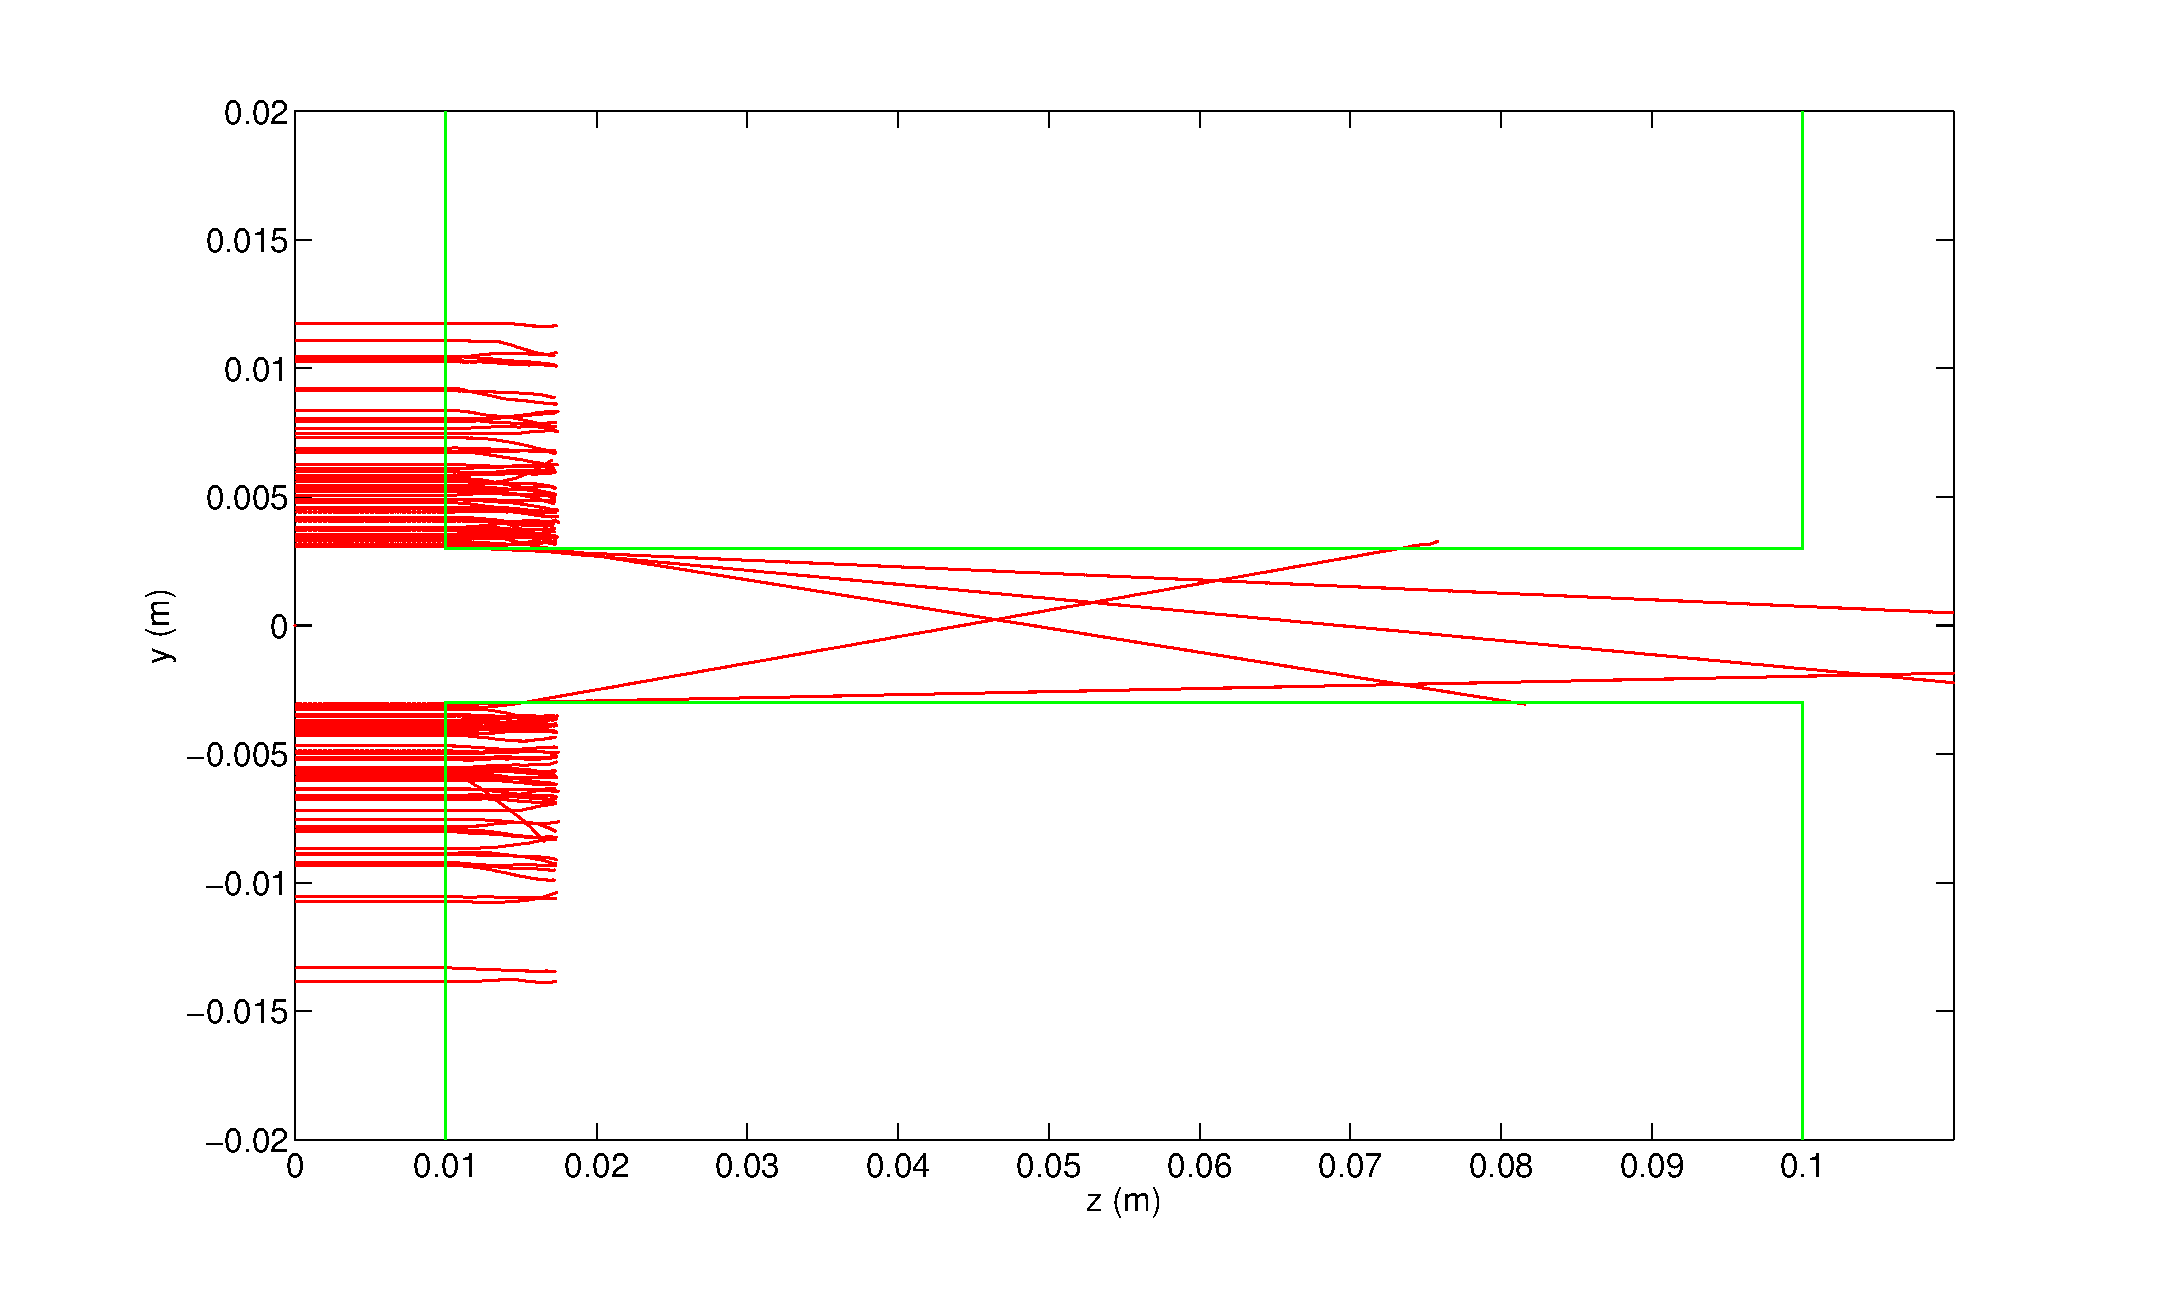
\includegraphics[width=0.9\linewidth]{trace3}
\end{figure}
 %\end{block}
\end{frame}


\begin{frame}{Beyond no-Colissions: Particle Matter Interaction cont.}{}
 
\begin{figure}[htb]
   \centering
  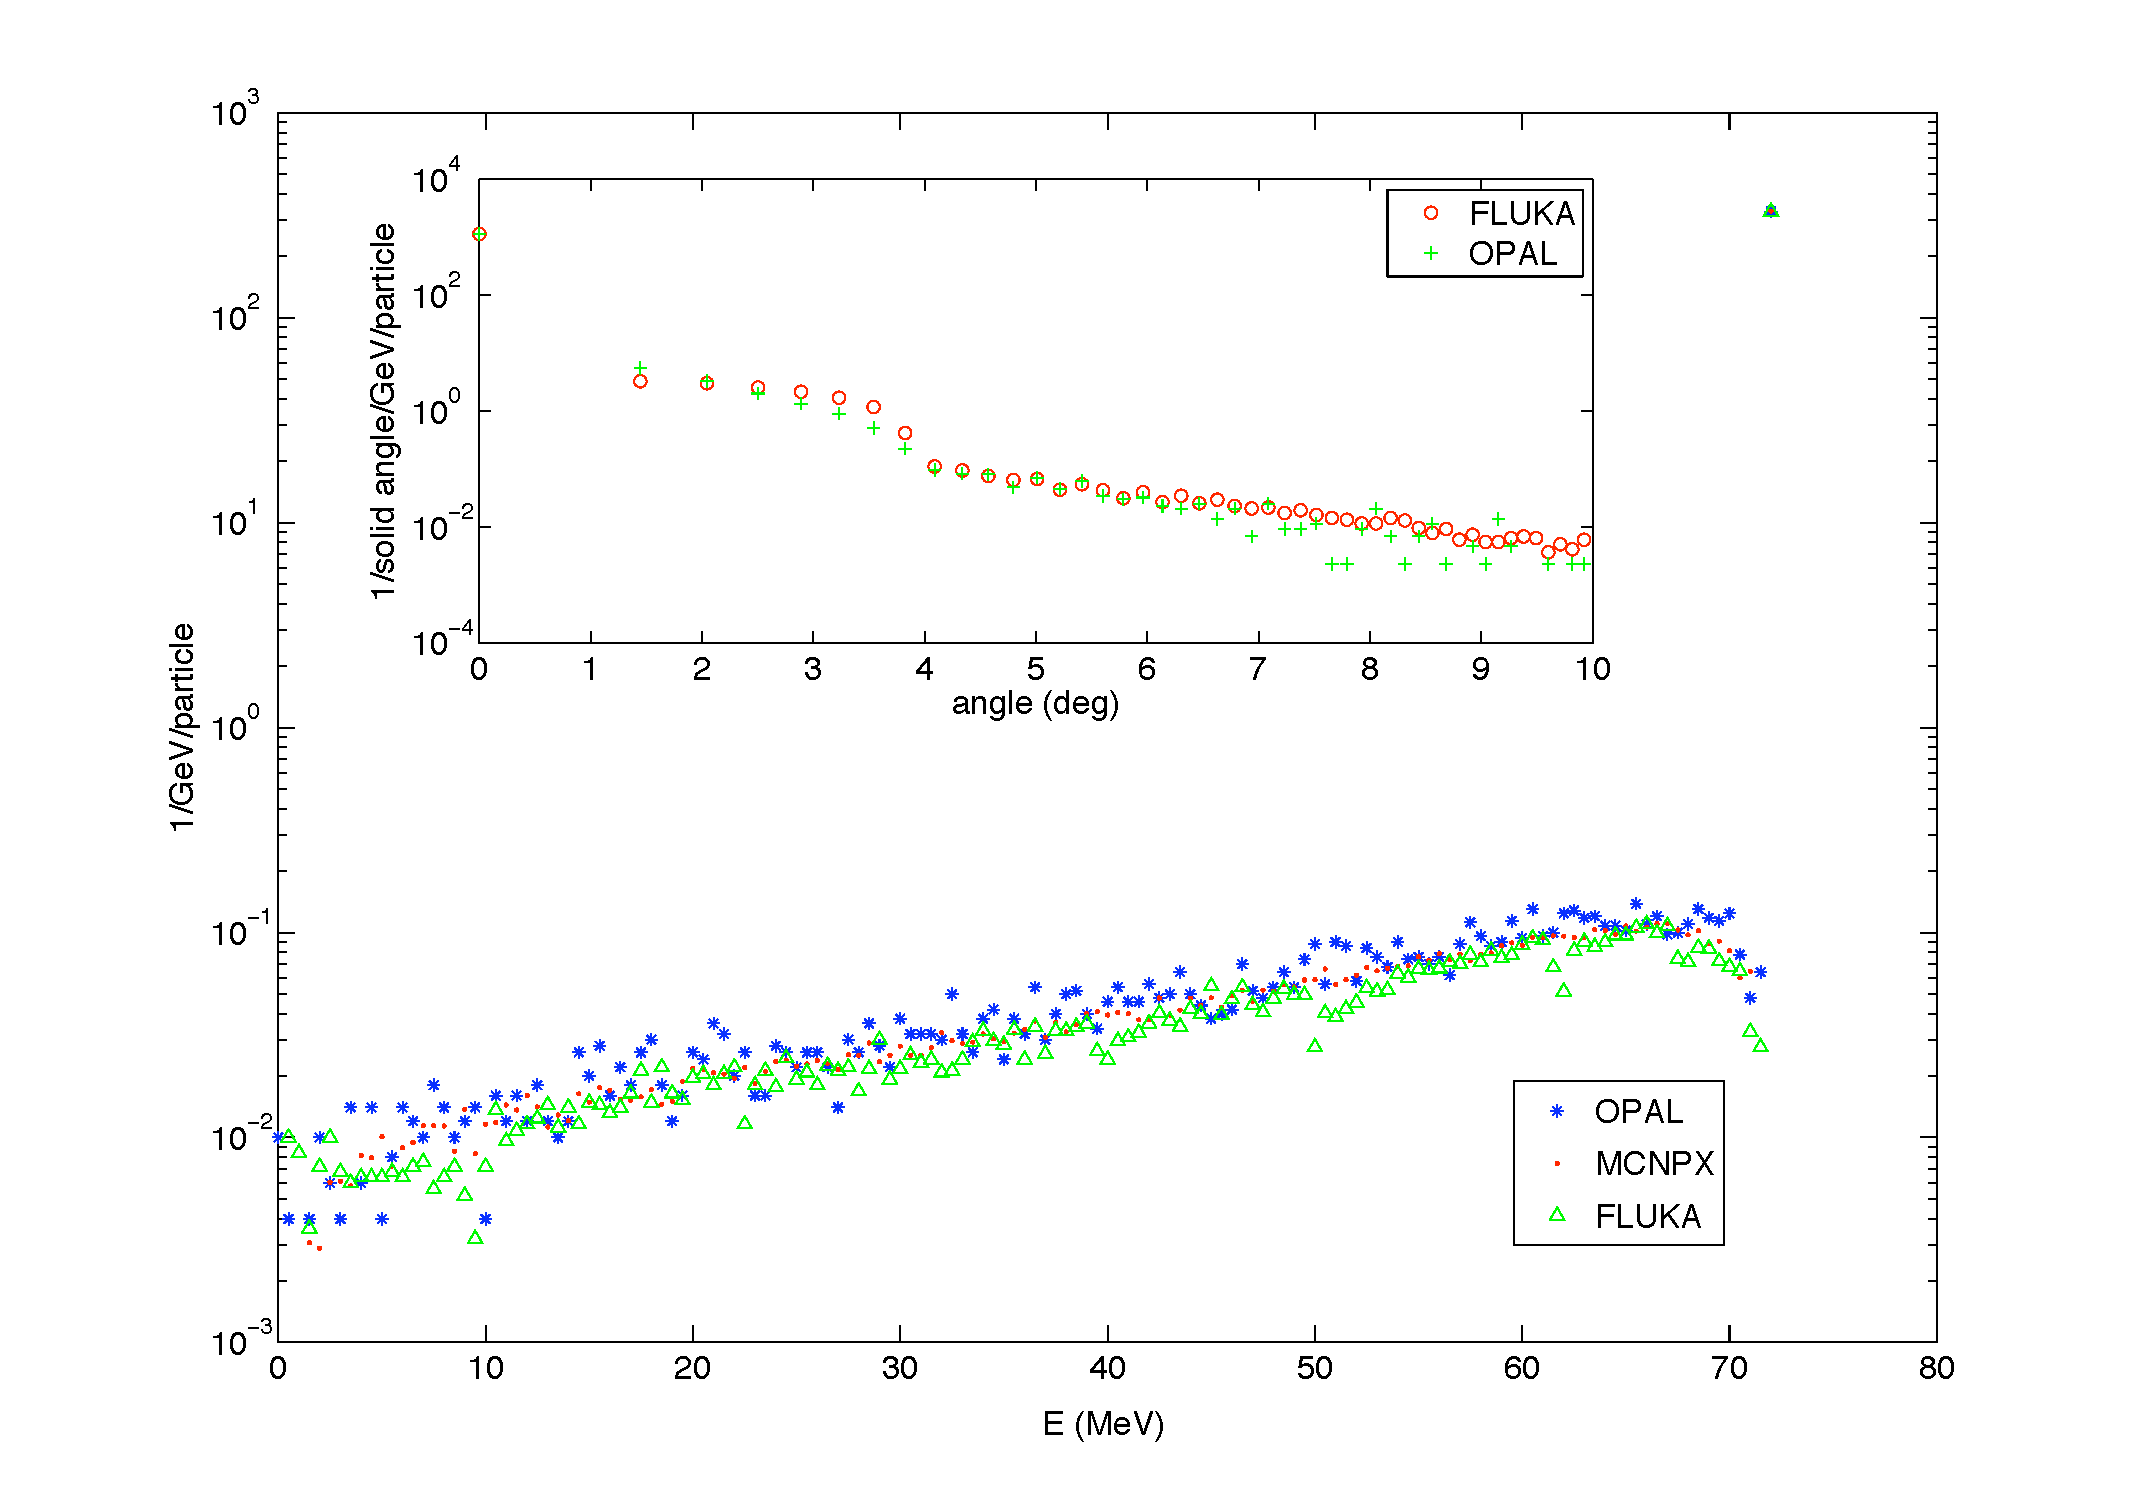
\includegraphics[width=0.9\linewidth]{spectandscatter}
 \end{figure}

\end{frame}





\begin{frame}{\opal in a Nutshell} {}
\begin{alertblock}{}  
 \opal is a tool for charged-particle optics in large
accelerator structures and beam lines including 3D space charge
\end{alertblock}
\begin{block}{Some of the features}  
\begin{itemize}
\item \opal is built from the ground up as a parallel application exemplifying the fact that HPC (High Performance Computing) 
is the third leg of science, complementing theory and the experiment
\item  \opal runs on your laptop as well as on the largest HPC clusters
\item \opal uses the \mad language with extensions
\item \opal (and all other used frameworks) are written in C++ using OO-techniques, hence \opal\ is very easy to extend.
\item Documentation is taken very seriously at both levels: source code and user manual (\url{ http://amas.web.psi.ch/docs/index.html})
\item Regression tests running evert day on the head of the repository
\end{itemize}
\end{block}
\end{frame}


\begin{frame}[fragile]
\frametitle{Sketch of an inputfile} 
%\framesubtitle{Sketch of an inputfile - \opalt}
%\begin{block}{}
\begin{verbatim}
Option, PSDUMPLOCALFRAME=TRUE;
Option, STATDUMPFREQ=1;
Option, REPARTFREQ=10;

Edes=.072;
gamma=(Edes+PMASS)/PMASS;
beta=sqrt(1-(1/gamma^2));

....

ring: Cyclotron, TYPE="RING", CYHARMON=6, PHIINIT=0.0,
			PRINIT=-0.000174, RINIT=2130.0,
			SYMMETRY=8.0, RFFREQ=frequency,
			FMAPFN="s03av.nar";

\end{verbatim}
%\end{block}
\end{frame}


\begin{frame}{\opal has a Layered Architecture} {}
\begin{figure}[htb]
\begin{center}
 \begin{tikzpicture}[scale=0.8, transform shape]
    \footnotesize
      \begin{scope}[shape=rectangle,rounded corners,minimum width=3.0cm,minimum height=0.5cm,fill=yellow,text centered]
      
      \draw[rounded corners, draw=green!40, thick, fill=green!25, opacity=0.5, text centered] (-1.55, 1.31) rectangle (8.55,-0.31) node[black, thick, anchor=center, opacity=1., font=\Large] at (3.5, 0.5) {\opal};
      \node[fill= green!40] (0_00) at (0.0,1.0) {MAD-Parser};
      \node[fill= green!40] (0_00) at (3.5,1.0) {Flavors: t,Cycl,Envelope};
      \node[fill= green!40] (0_00) at (7.0,1.0) {Optimization};
      \node[fill= green!40] (0_00) at (0,0.0)   {Solvers: Direct, Iterative};
      \node[fill= green!40] (0_00) at (3.5,0.0) {Integrators};
      \node[fill= green!40] (0_00) at (7.0,0.0) {Distributions};

       \draw[rounded corners, draw=red!45, thick, fill=red!25, opacity=0.5, text centered] (-1.55, -0.69) rectangle (8.55,-3.81) node[black, thick, anchor=center, opacity=1.0, font=\Large] at (3.5, -2.25) {\ippl};
       \node[fill= red!45] (q_00) at (0,-1) {FFT};
       \node[fill= red!45] (q_01) at (3.5,-1) {D-Operators};
       \node[fill= red!45] (q_02) at (7,-1) {NGP,CIC, TSI};
       \node[fill= red!45] (q_10) at (0,-1.75) {Fields};
       \node[fill= red!45] (q_11) at (3.5,-1.75) {Mesh};
       \node[fill= red!45] (q_12) at (7,-1.75) {Particles};
       \node[fill=red!45] (q_20) at (0,-2.75) {Load Balancing};
       \node[fill=red!45] (q_21) at (3.5,-2.75) {Domain Decomp.};
       \node[fill=red!45] (q_22) at (7,-2.75) {Message Passing};
       \node[fill=red!45] (q_20) at (0,-3.5) {STL};
       \node[fill=red!45] (q_21) at (3.5,-3.5) {PETE};
       \node[fill=red!45] (q_22) at (7,-3.5) {Polymorphism};

       \node[rotate=90,minimum width=1.7cm,fill=gray] (bla) at (-1.9,0.49){\textcolor{white} {\classic}};
       \node[rotate=90,minimum width=3.15cm,fill= magenta] (bla) at (-1.9,-2.225){\textcolor{white}{\hfifehut}};
       \node[fill=blue!65,minimum width=10.75cm] (q_23) at (3.25,-4.25) {\textcolor{white}{Trilinos \& GSL}};

      \end{scope}
 \end{tikzpicture}
%\caption{The \opal\ software structure}
\label{fig:opalstr}
\end{center}
\end{figure}
 \vspace{-0cm}
   \begin{itemize}
   \item {\bf\color{green}  {\bf \opal Object Oriented Parallel Accelerator Library}}
   \item {\color{red} $\text{IP}^{2}L$ {\bf Independent Parallel Particle Layer}}
   \item {\color{gray}  {\bf Class Library for Accelerator Simulation System and Control}}
   \item  {\bf\color{magenta} {\bf \hfifehut for parallel particle and field I/O (HDF5)}}
   \item {\bf\color{blue!65} {\bf Trilinos} http://trilinos.sandia.gov/}
  \end{itemize}
 \end{frame}



\begin{frame}{Maxwell's Equation in the Electrostatic approximation} {}
\begin{block}{}
In 3D Cartesian coordinates, the solution of the Poisson equation at point $\bs{x}$ can be expressed by 
\begin{equation}\label{eq:Poten}
  \phi(\bs{x})= \frac{1}{4\pi\varepsilon_0}\int{G(\bs{x},\bs{x}')\rho(\bs{x},\bs{x}')d\bs{x}'}
\end{equation}
with $G$ the 3D Green function 
\begin{equation}\label{eq:Green}
  G(\bs{x},\bs{x}')= \frac{1}{\sqrt{(\bs{x}-\bs{x}')^2}}
\end{equation}
assuming open boundary conditions.
The typical steps of calculating space charge fields using the parallelized Hockney's FFT algorithm.
\end{block}
 \end{frame}



	\begin{frame}
		\frametitle{Discretization: Particle-in-cell (PIC) }

		\begin{block}{}
        \begin{minipage}[b]{0.75\textwidth}
		\begin{itemize}
			\item Interpolate individual particle charges to the grid
			\item Solve the Poisson equation on the mesh in a Lorentz frame
			\item Finite-Difference Schemes or Direct  Solver (FFT)
		\end{itemize}
        \end{minipage}
        \begin{minipage}[b]{0.15\textwidth}
        \centering
		\begin{tikzpicture}[scale=1.0,transform shape,node distance=1cm]	
			\draw[very thin,color=gray,step=2cm] (-0.2,-0.2) grid (2.2,2.2);
			\fill[color=blue,opacity=0.6] (1.3,0.5) circle (3pt);
			\fill[color=red,opacity=0.6] (2.0,2.0) circle (1pt);
			\fill[color=red,opacity=0.6] (2.0,0.0) circle (1pt);
			\fill[color=red,opacity=0.6] (0.0,0.0) circle (1pt);
			\fill[color=red,opacity=0.6] (0.0,2.0) circle (1pt);
			
            \path[style=thick,dashed, ->] (1.3,0.5) edge (2.0,2.0);
            \path[style=thick,dashed, ->] (1.3,0.5) edge (2.0,0.0);
            \path[style=thick,dashed, ->] (1.3,0.5) edge (0.0,2.0);
            \path[style=thick,dashed, ->] (1.3,0.5) edge (0.0,0.0);

		\end{tikzpicture}

        \end{minipage} 
		\end{block}

		\vspace{0.5cm}
	
     

	\end{frame}





\begin{frame}
		\frametitle{Direct Poisson Solver}
		\begin{block}{}
		\begin{algorithmic}[1]
		    \STATE \textbf{procedure} 3DSpaceCharge(In: $\rho$, $G$, Out: $\bs{E_{sc}}$,$\bs{B_{sc}}$)
       \STATE Create 3D rectangular grid which contains all particles, % and doubled it in each dimension, 
       \STATE Interpolate the charge $q$ of each macro-particle to nearby mesh points to obtain $\rho^D$, 
       \STATE Lorentz transformation to obtain $\rho^D$ in the beam rest frame $\bs{S}_{\RM{beam}}$,
       \STATE FFT $\rho^D$ and $G^D$ to obtain $\widehat{\rho}^D$ and $\widehat{G}^D$,
       \STATE Determine $\widehat{\phi}^D$ on the grid using $\widehat{\phi}^D = \widehat{\rho}^D \cdot \widehat{G}^D$,
       \STATE Use FFT$^{-1}$ of $\widehat{\phi }^D$ to obtain $\phi^D$,
       \STATE Compute $\bs{E}^D= -\nabla \phi^D$,
       \STATE Interpolate $\bs{E}$ at the particle positions $\bs{x}$ from $\bs{E}^D$,
       \STATE Perform Lorentz back transform to obtain $\bs{E_{\RM{sc}}}$ and $\bs{B_{\RM{sc}}}$ in  frame $\bs{S}_{\RM{local}}$ and transform back  to $\bs{S}_{\RM{lab}}$.
       \STATE \textbf{end procedure}	
			
					\end{algorithmic}
		%\end{algorithm}
		\end{block}
\alert{\ippl: parallel FFT, domain decomposition (grids, particles), ghost cells and $\vec{h}(t)$}
	\end{frame}


\begin{frame} 
  \frametitle{Parallel Scalability: \small{Test on Cray XT3 at CSCS, Switzerland}}
  \begin{columns}
    \begin{column}{4.cm}
      \scriptsize
      \begin{block}{Setup}
        \begin{itemize}
        \item  \alert{$10^6$} particles, 
        \item 3D FFT on a  \alert{$64^3$} grid,
	\item \alert{2D} domain decomposition
	\item Track  \alert{200} time steps
        \item Gaussian distribution
	\item Dump data into \alert{single} H5Part file every 10 steps
        \end{itemize}
      \end{block}
      
      \begin{block}{Observations}
        \begin{itemize}
        \item The code scales well
	\item Good load-balancing
	\item I/O time is increasing 
        \end{itemize}
      \end{block}
    \end{column}
    \begin{column}{6.5cm}
%    \begin{block}{}    
      \includegraphics[width=0.95\linewidth]{Timing64mesh}
      \center Time to solution is reduced approximately by a factor of \alert{60}, (256P Vs 1P).
   % \end{block}  
    \end{column}
  \end{columns}
\end{frame}


\begin{frame}{\opal Parallel Scaling on Cray XT5 at CSCS}{Direct FFT Based Solver}
 \vspace{-3mm}  
   \begin{columns}
    \begin{column}{11.0cm}
      \scriptsize
%      \begin{block}{Production Run Setup}
        \begin{itemize}
       \item Tracking $10^8$ particles 
        \item 3D FFT on a $1024^3$ grid
        \item Gaussian distribution
       \end{itemize}
    
        
    %  \end{block}
    
    \end{column}
%    \begin{column}{7.0cm}
%%    \begin{block}{}
%      \includegraphics[scale=0.35]{figures/drift2c1} 
% %   \end{block}
%    \end{column}
   
  \end{columns}
  \vspace{-5mm}
  \includegraphics[scale=0.32]{drift2c1}
%    \begin{block}{Observation}
%      \begin{center}
%         \alert{Time to solution reduced approximately by a factor of 100}
%        \end{center}
%     \end{block}
\end{frame}






%\frame{
%   \frametitle{870 keV Injection Line}
%  \framesubtitle{\alert {Simulation} and \alert{measurement} DC beam 870 keV}
% 
%{\bf Find $\mathcal{D}_{start}$ and $\nu_e$ by $min(F)$:} $F =\sum_{n=1}^{\#monitors}{(\rms{\mathcal{X}}_{mea}(s_n)-\rms{\mathcal{X}}_{sim}(s_n))^2} .$
% %beamline_without_accelerator_870keV
%    \begin{center}
%     %\begin{overprint}
%      %\includegraphics<1>[keepaspectratio=true,width= 0.50\linewidth,angle=90]{870line} 
%      \includegraphics<1>[keepaspectratio=true,width= 0.45\linewidth,angle=0]{MWP30}
%      %\end{overprint}
% \end{center}
%}



%\frame{
%\frametitle{870 keV Injection Line}
%\framesubtitle{\alert{Buncher}}

%\includemovie[
%poster,
%text=(870 keV Buncher),
%mouse,
%repeat
%]{
%.8\linewidth
%}{
%.6\linewidth
%}{movieBuncher-2.mpeg}
%}

%\frame{ 
%
%  \frametitle{PSI Injector II}
%  \framesubtitle{\alert{Center Region Collimation}}
%  \begin{columns}
%    \begin{column}{6.0cm}
%     \includegraphics[width=0.5\linewidth]{Inj2xz-Col}
%    \end{column}
%    
%    \begin{column}{6.0cm}
%      \begin{overprint}
%      \includegraphics<1>[width=0.9\linewidth]{INJII}
%       \includegraphics<2>[keepaspectratio=true,width=0.5\linewidth,angle=-90]{inj2-Coll}
%  \end{overprint}
%    \end{column}
%  \end{columns}  

%  \begin{block}{Conclusion} 
%    In Injector2, \sce help to develop a very compact stable core in the first several turns for more than 1mA beam.
%  \end{block}

%}

\frame{
  \frametitle{PSI 590 MeV Ring - last 8 truns} 
 \framesubtitle{\alert{Compare with measured profiles}}


%  \begin{block}{Start-to-end RMS sizes comparison of a 3MeV beam}  
    \includegraphics[width=0.9\linewidth]{rre4v0120all}
   
 % \end{block}
}



\section{GPU and Many Core Considerations}

\frame{
\frametitle{How to best port \opal onto GPU and/or Many Core Architectures?}
\alert{}
\begin{block}{Investment protection}
[Bordawekar 2010] Believe it or Not! Multi-core CPUs Can Match GPU Performance for FLOP-intensive Application!, 
IBM RC24982 (W1004-095)
\begin{itemize}
\item CM5 of Thinking Machine
\item Road Runner (IBM Cell)
\item but now .... things getting maybe better!
\end{itemize}
\end{block}
\opal is a very complex and large parallel OO-Code
\begin{itemize}
\item \opal is memory bound $\mathcal{O}(100)$ Bytes per particle
\item need Double precision
\item I/O of large data sets (HDF5 based) is very important
\item complicated geometries will be very important in the near future
\end{itemize}
}

\frame{
\frametitle{Memory Bandwidth Hierarchie } 
\begin{center}
\includegraphics[width=0.75\linewidth]{GPU-ARCH1}
\vspace{-3.5mm}
\begin{alertblock}{}
\begin{center}
$ B_{mg} > B_m > B_n $ {\bf and}  $B_n > B_g$ \alert{what about} $B_f$?
\end{center}
\end{alertblock}
\end{center}
}


	\begin{frame}
	\frametitle{Memory Bandwidth Hierarchie cont. } 
	
  \begin{center}
          \rowcolors{1}{blue!20}{blue!5}
          \begin{tabular}{cccccc}
            \hline
             {\tiny /(GB/s)}& $B_{mg}$ & $B_m$ & $B_n$ & $B_g$ & $B_f$ \\
            \hline
            IBM BG-P & --- & $7.6 \dots 13$ &$5.1$& --- & --- \\
            \hline
            Cray XT5 & --- & $19 \dots 25.6$ & $ \mathcal{O}(10)$ & --- & 10 \\
            \hline
            NVidia & $78 \dots 144$  & --- & --- & $5$ & --- \\
            \hline
          \end{tabular}
        \end{center}

	\begin{columns}
		\begin{column}{5.5cm}
		\begin{center}
\includegraphics[width=1.0\linewidth]{GPU-ARCH1}
\end{center}	
		\end{column}
		\begin{column}{5.5cm}
\begin{itemize}
\item $B_f$ with $\mathcal{O}(10000)$ cores on Jaguar
\item $B_g$ on 16 lane PCI-E Gen-2 using two different NVidia Tesla cards (one a GTX280 and the other is a Fermi card)
\item \alert{my primary concern is $B_g$}
\end{itemize}		
		\end{column}
	\end{columns}

(some of the data obtained from J. Shalf LBL)
		
	\end{frame}

 \begin{frame}[containsverbatim]{Choice: Ignore GPU}
\begin{itemize}
\item Continue with optimized pieces (FFT,Trilinos etc.) because it works
\begin{itemize}
\item automatically take advantages of new development like multi-core
\end{itemize}
\item Add may core support: multi threading \& OpenMP - MPI
\begin{itemize}
\item very promising, because of Expression Templates (PETE), here the expression is evaluated in the  assignment operator
\end{itemize}
\end{itemize}
Assume $A,B,C,D$ are vectors, we want to evaluate $D=A+B+C$
\begin{itemize}
\item The sole loop of the vector evaluation is contained in the assignment operator \begin{smallcode}
   template< typename R > 
   inline Vector& Vector::operator=( const R& rhs ) 
   { 
      for( unsigned int i=0; i<length_; ++i ) 
         p_[i] = rhs[i]; 
   }
\end{smallcode}
\item Very easy to parallelize on several levels
\end{itemize}

\end{frame}


\frame{
\frametitle{Choice: GPU light}
%\begin{block}{}
\begin{itemize}
\item Re-implement all the functionality of the kernel (solver,PIC,particle pusher) to \alert{one} GPU board
\item Limits us to small problem sizes and simple geometries
\begin{itemize}
\item limited memory on one GPU board 
\item PIC code implementation (Viktor K. Decyk) showing very good performance: {\em ... expect to achieve a factor of about 50-100 speedup over the Intel Nehalem} 
\end{itemize}
\end{itemize}
\begin{center}
\includegraphics[width=0.5\linewidth]{GPU-ARCH2}
\end{center}

%\end{block}
}

\frame{
\frametitle{Choices \opal on many GPU Boards} 
\vspace{-0.5mm}
\begin{itemize}
\item Scatter/Gather and particle integration on GPU
\item FFT on host
\item (potential) Problem: Load balancing i.e. $B_g$ limit
\includegraphics[width=0.6\linewidth]{GPU-ARCH3}
\item geometry handling ?
\end{itemize}
%\end{block}
}


\section{Conclusions \& Outlook}

\begin{frame}{Conclusion and  Outlook}{}

\begin{itemize}
\item GPU with DMA instead of PCI-E would be the ideal case of such kind of application
\item Depending on manpower/funding we will consider the described option GPU light:
\begin{center}
\includegraphics[width=0.5\linewidth]{GPU-ARCH2}
\end{center}
\item Explore Multi-Core among the line of Expression-Templates
\end{itemize}

\end{frame}

\frame{
\frametitle{Outlook: Dark Current \& Multipacting Simulations}
\includemovie[
poster,
text=(Dark Current),
mouse,
repeat
]{
.8\linewidth
}{
.6\linewidth
}{Movies/dc-1.avi}

{\tiny For \oursolver\ see: Adelmann/Arbenz/Ineichen, J. Comp. Phys., 229, 4554-4566, 2010}

}


\end{document}





